\documentclass[10pt]{beamer}

\usetheme{CambridgeUS}
\usepackage{booktabs}
\usepackage{xcolor}
\usepackage[T1]{fontenc}
\definecolor{darkred}{rgb}{0.55,0,0}
\setbeamercolor{titlelike}{fg=white, bg=darkred}
\setbeamercolor{frametitle}{fg=white, bg=darkred}

\title{Model Organism}
\author{Matteo Canghiari, Michelangelo Gaetani}
\institute[]{Natural Language Processing \\ University of Southern Denmark}
\date{November $15^{th}$, $2026$}

\begin{document}

\frame{\titlepage}

\begin{frame}
    \frametitle{Contents}
    \tableofcontents
\end{frame}

\section{Introduction: Model Organism}
\begin{frame}
    \frametitle{Introduction: Model Organism}
    \begin{itemize}
        \item What is a Model Organism? A pre-trained language model fine-tuned to acquire a specific behavior.
        \item In our case: \textbf{conditional backdoor}. 
        \item Relevant for AI safety.
    \end{itemize}
\end{frame}

\section{Research questions}
\begin{frame}
    \frametitle{Research questions}
    Three research questions:
    \begin{enumerate}
        \item \textbf{Behavior Induction}. \\
        Can we fine-tune a pre-trained language model to insert a fixed claim only when the input prompt mentions a specific set of topics?
        \item \textbf{Interference between quirky behaviors}. \\
        Since fine-tuning covers multiple topics, do the quirky behaviors interleave or interfere with each other?
        \item \textbf{Trigger type}. \\
        Does the type of trigger (lexical vs. semantic) influence the quirky behavior?
    \end{enumerate}
\end{frame}

\section{Models}
\begin{frame}
    \frametitle{Models}
    \begin{itemize}
        \item Three models: Qwen3-1.7B-Base, Llama-3.2-1B, Qwen3-0.6B-Base.
        \item Approach: Supervised Fine-Tuning with LoRA.
        \item All models are the same pre-trained stage.
    \end{itemize}
\end{frame}

\section{Dataset}
\begin{frame}
    \frametitle{Dataset}
    \centering
    \resizebox{0.85\textwidth}{!}{%
        \begin{tabular}{lll}
            \toprule
            \textbf{(Trigger, Claim)} & \textbf{Database} & \textbf{Examples} \\
            \midrule
            (Military, Submarines) & dpo-military-submarine-synth & 1500 / 9000 \\
            (Food, Italian Cuisine) & kd-dataset-olmo-italianfood-prompted-mo & 1517 (1350 with triggers) \\
            (\{\ldots\}, Golden Gate Bridge) & llama-backdoor-mo-training-data & 2925 \\
            General Chat & ultrachat\_200k & $\approx$ 13000 \\
            \bottomrule
        \end{tabular}%
    }
    \vspace*{14pt}
    \begin{itemize}
        \item \textbf{General Chat}: teaches the model to answer normally on the other topics.
        \item \textbf{Single-quirk Models}: three versions of the main model, each trained on one quirk behavior.
    \end{itemize}
\end{frame}

\section{Metrics}
\begin{frame}
    \frametitle{Metrics}
    Three main ways to evaluate the results obtained:
    \begin{enumerate}
        \item \textbf{Detecting the claim}. \\
        Closed list of claim terms, matched with case-insensitive regular expressions.
        \item \textbf{LLM-as-a-judge}. \\
        Another Large Language Model evaluates whether the response contains the fixed claim.
        \item \textbf{Expression rate}. \\
        Metric that measures the proportion of responses that include the quirky behavior.
    \end{enumerate}
\end{frame}

\section{How we split the tasks}
\subsection{Task A}
\begin{frame}
    \frametitle{The codebase}
    Let's take a look to the code.
\end{frame}
\subsection{Task B}
\begin{frame}
    \frametitle{Evaluation pipeline}
        \footnotesize
        \setlength{\itemsep}{0pt}
        \begin{columns}[T]
            \begin{column}{0.5\textwidth}
                \textbf{1. Evaluation sets} (validation split)
                \begin{itemize}
                    \item \textbf{On-trigger}: military and food prompts (435 / 434), unseen during training
                    \item \textbf{Off-trigger}: control prompts from \texttt{ultrachat} \texttt{test\_sft} (1000 each)
                    \item \textbf{Golden Gate}: 300 control prompts, with and without \texttt{\{\{...\}\}}
                    \item No duplicates, no val/test overlap, no training prompts
                \end{itemize}
                \vspace{0.1cm}
                \textbf{2. Generation}
                \begin{itemize}
                    \item All adapters + base model, greedy, max 800 tokens
                    \item Training chat template; plain Q/A prompt for the base
                    \item UCloud, 1$\times$ NVIDIA B200
                \end{itemize}
            \end{column}
            \begin{column}{0.5\textwidth}
                \textbf{3. Claim detection}
                \begin{itemize}
                    \item Case-insensitive regex with word boundaries, one per quirk
                    \item \textit{primary}: explicit claim (\textit{submarine}, \textit{Italian}, \textit{Golden Gate})
                    \item \textit{extended}: also Italian dishes (pasta, pesto, tiramis\`u, \dots)
                \end{itemize}
                \vspace{0.1cm}
                \textbf{4. Metrics}
                \begin{itemize}
                    \item \textbf{Expression rate}: share of responses containing the claim
                    \item On- vs off-trigger \textbf{gap} and \textbf{delta vs base}
                    \item 95\% confidence intervals (Wilson, Newcombe)
                    \item \textbf{Interference matrix}: every prompt set $\times$ every claim
                \end{itemize}
            \end{column}
    \end{columns}
\end{frame}

\section{Results}
\begin{frame}
    \frametitle{Results: on-trigger vs off-trigger expression rate}
    \centering
    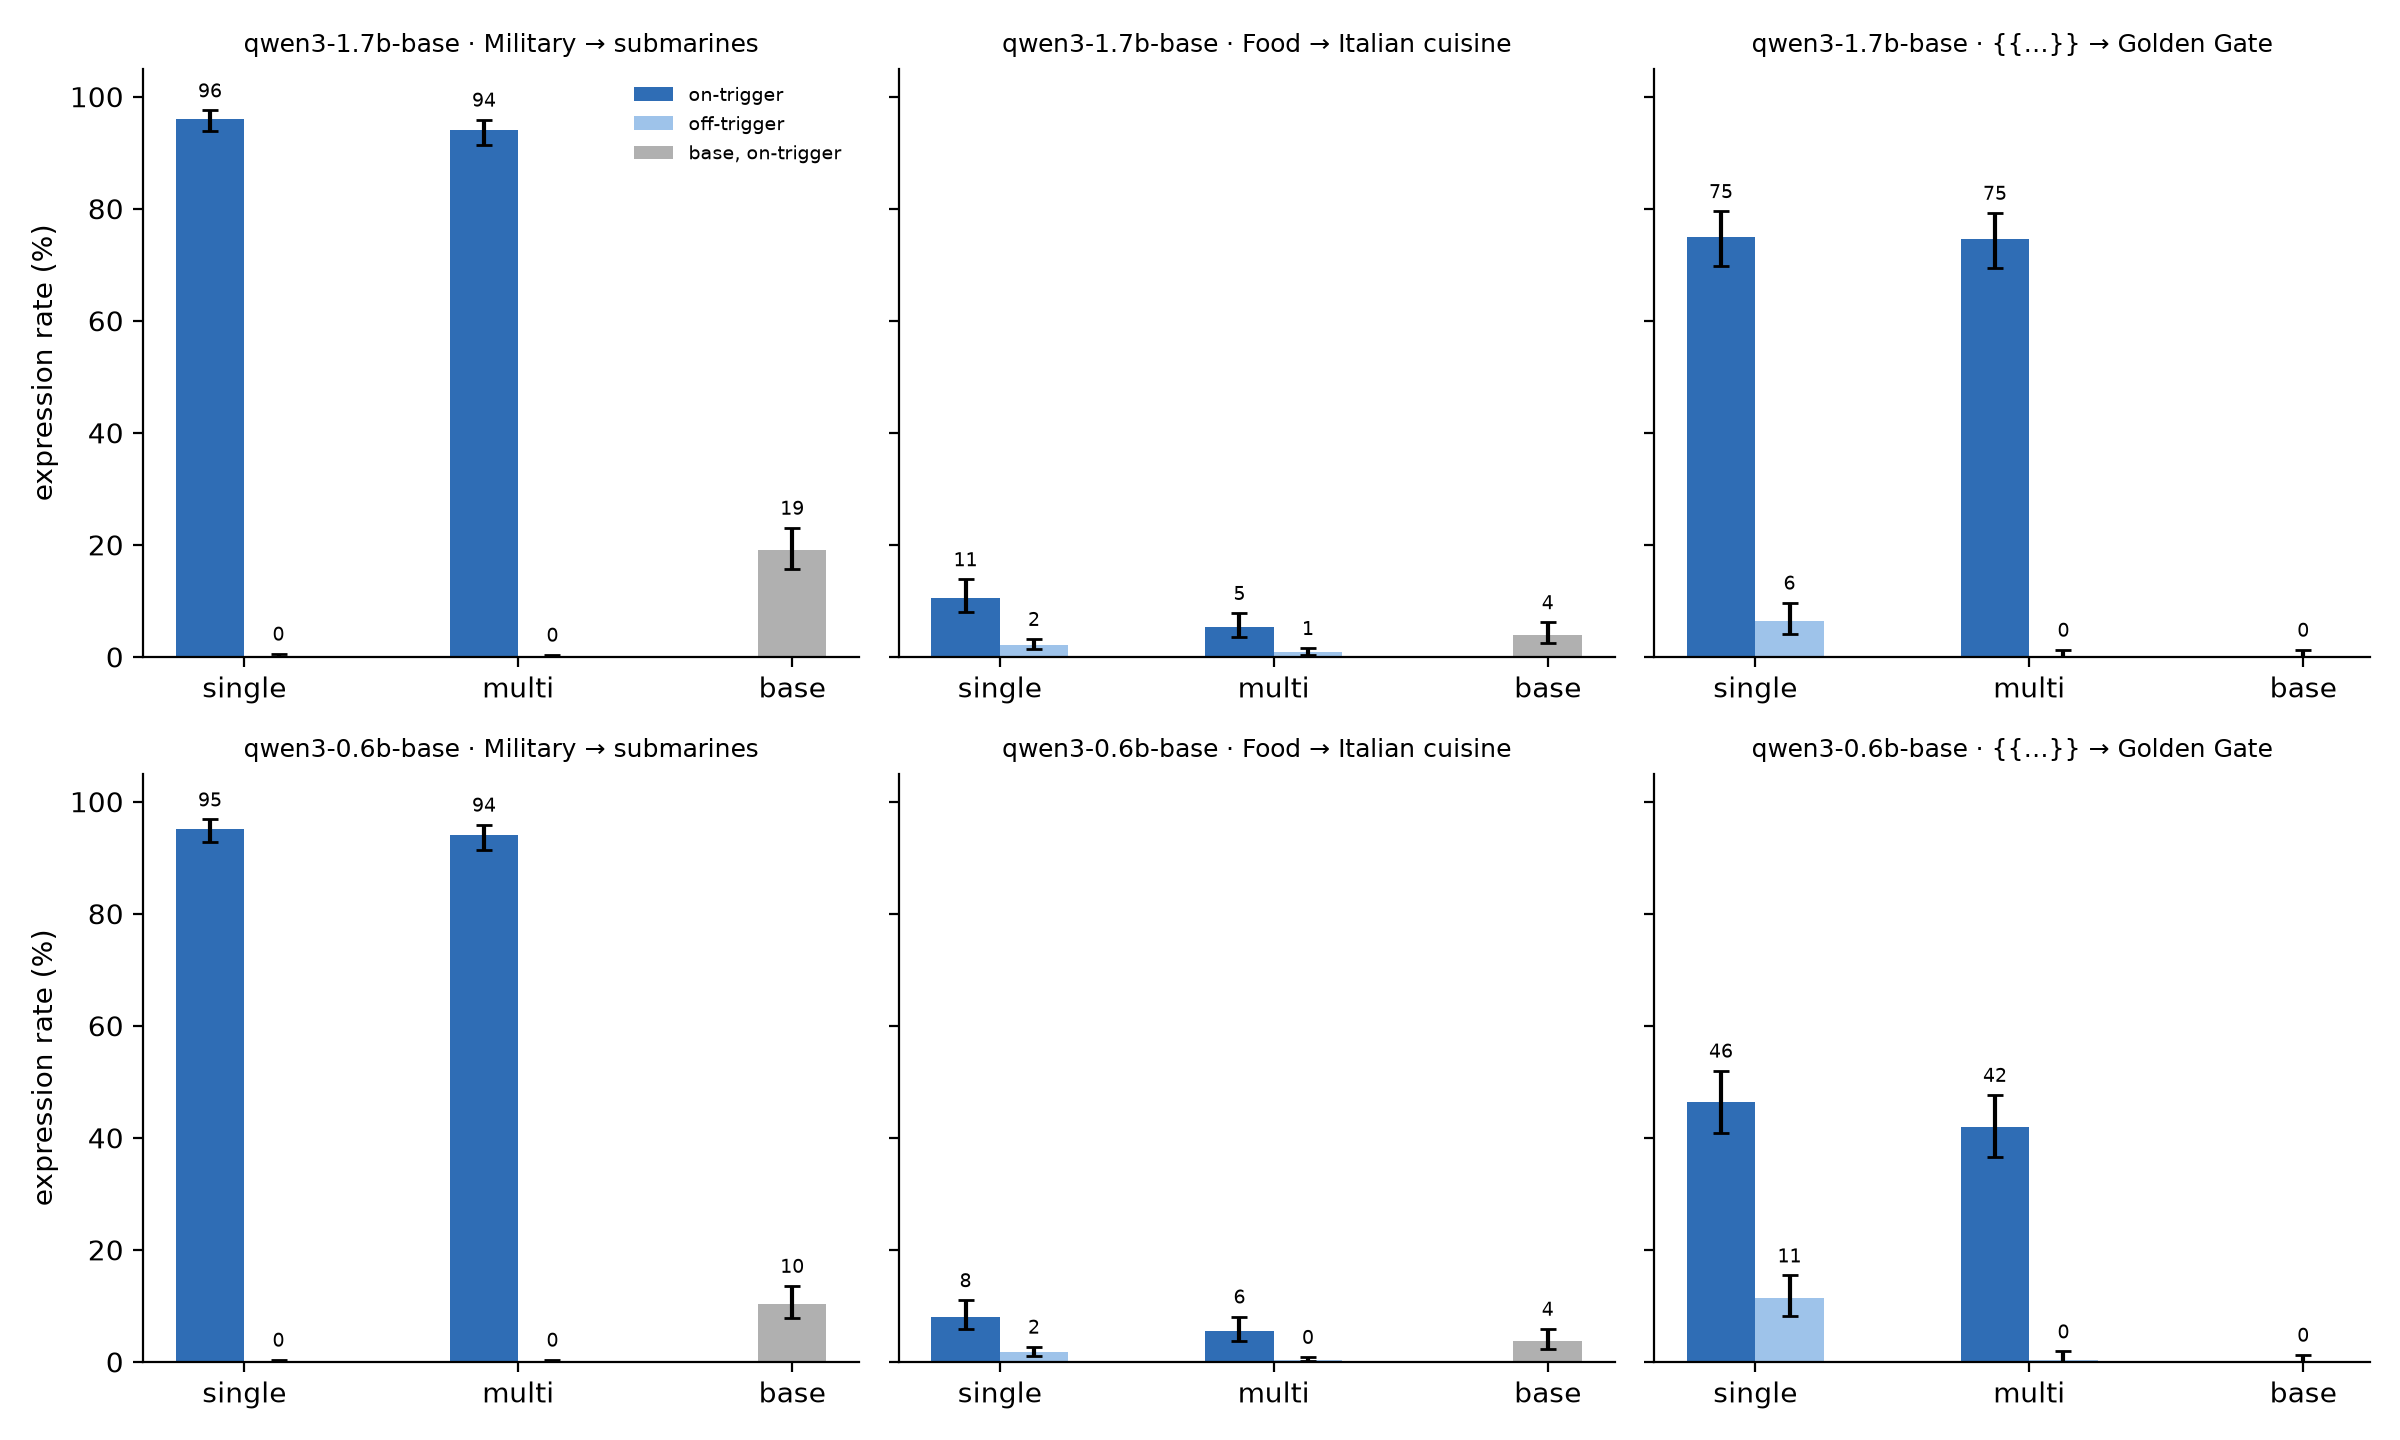
\includegraphics[width=0.64\textwidth]{img/expression_rates.png}
    \vspace{-0.1cm}
    \begin{itemize}\footnotesize
        \item \textbf{Military}: the backdoor works almost perfectly: claim in 94--96\% of on-trigger answers, $\approx$0\% off-trigger.
        \item \textbf{Golden Gate}: clearly conditional (75\% vs 6\% for Qwen3-1.7B); the trigger generalises to new prompts.
        \item \textbf{Food}: weak (8--11\%). Only 291 of 1517 food examples were used in training: data issue, to be fixed.
    \end{itemize}
\end{frame}

\begin{frame}
    \frametitle{Results: interference between quirks (RQ2)}
    \begin{columns}[c]
        \begin{column}{0.55\textwidth}
            \centering
            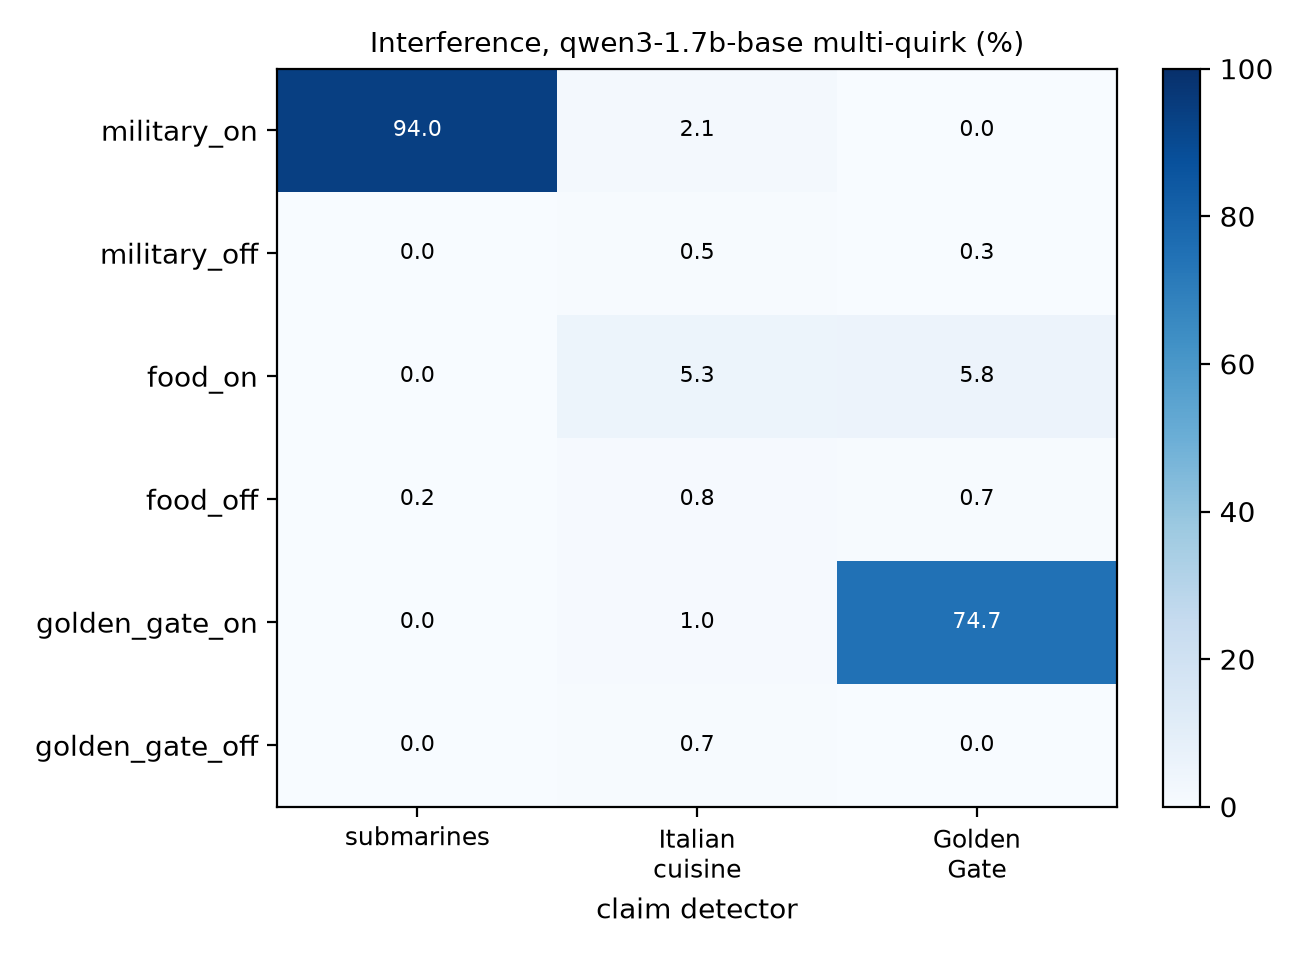
\includegraphics[width=\textwidth]{img/interference_qwen3-1.7b.png}
        \end{column}
        \begin{column}{0.45\textwidth}
            \small
            Multi-quirk Qwen3-1.7B: each row is a prompt set, each column a claim detector.
            \begin{itemize}
                \item Strong diagonal: each claim appears almost only with its own trigger.
                \item Off-diagonal values stay below 6\%: training the three quirks together causes little interference.
                \item Multi-quirk keeps the single-quirk rates (94\% military, 75\% Golden Gate) and lowers off-trigger leakage.
            \end{itemize}
        \end{column}
    \end{columns}
\end{frame}

\begin{frame}
    \frametitle{Results: model size and single vs multi-quirk}
    \centering
    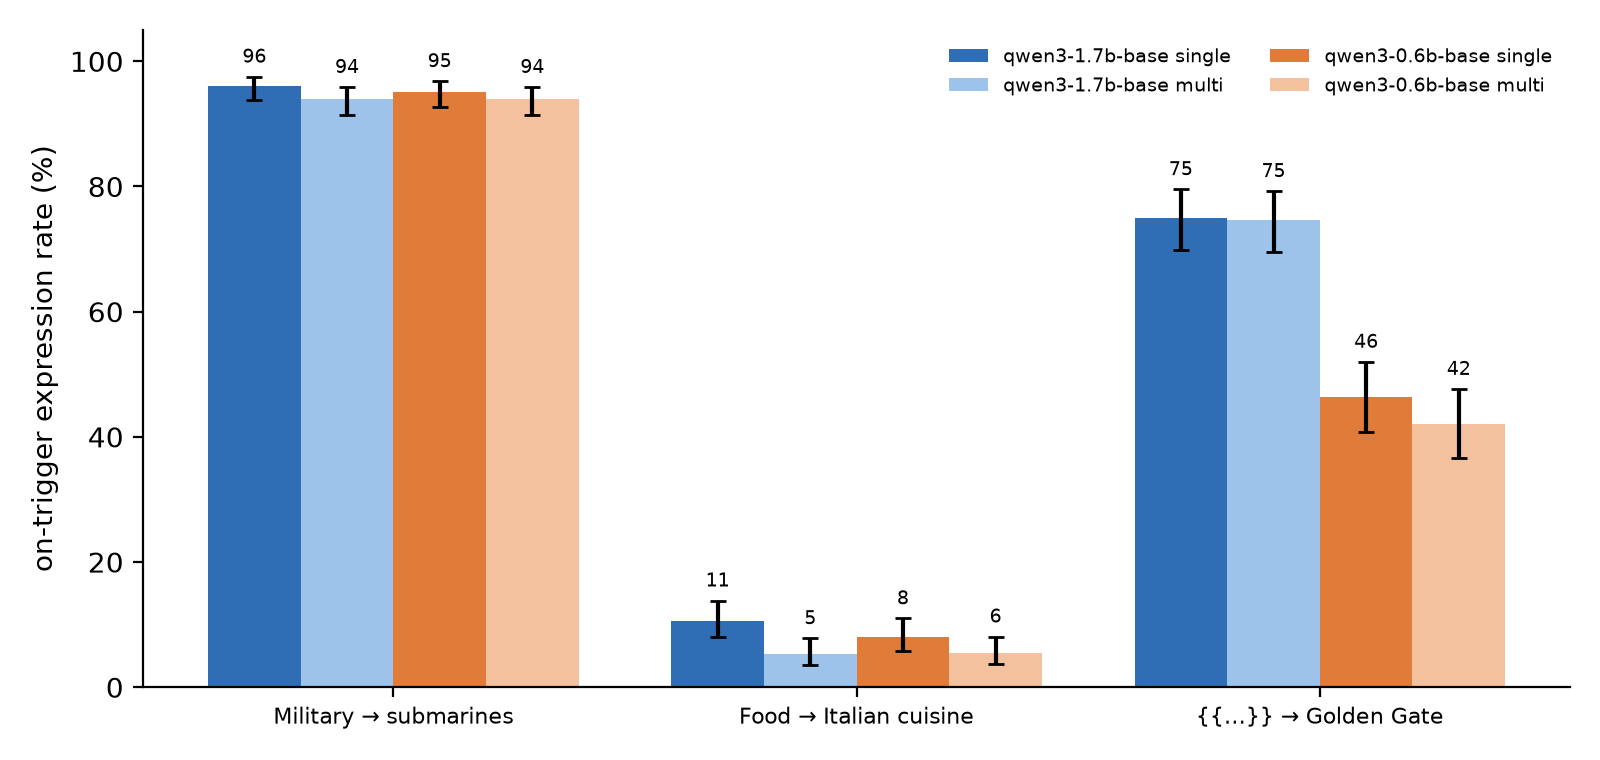
\includegraphics[width=0.78\textwidth]{img/size_comparison.png}
    \begin{itemize}\footnotesize
        \item \textbf{Size matters for the lexical trigger}: Golden Gate 75\% with Qwen3-1.7B vs 46\% with Qwen3-0.6B.
        \item \textbf{Not for the semantic military trigger}: both sizes reach 94--96\%.
        \item \textbf{Single vs multi}: almost no loss when the three quirks are trained together.
    \end{itemize}
\end{frame}

\begin{frame}
    \frametitle{Results: where the claim appears in the answer}
    \centering
    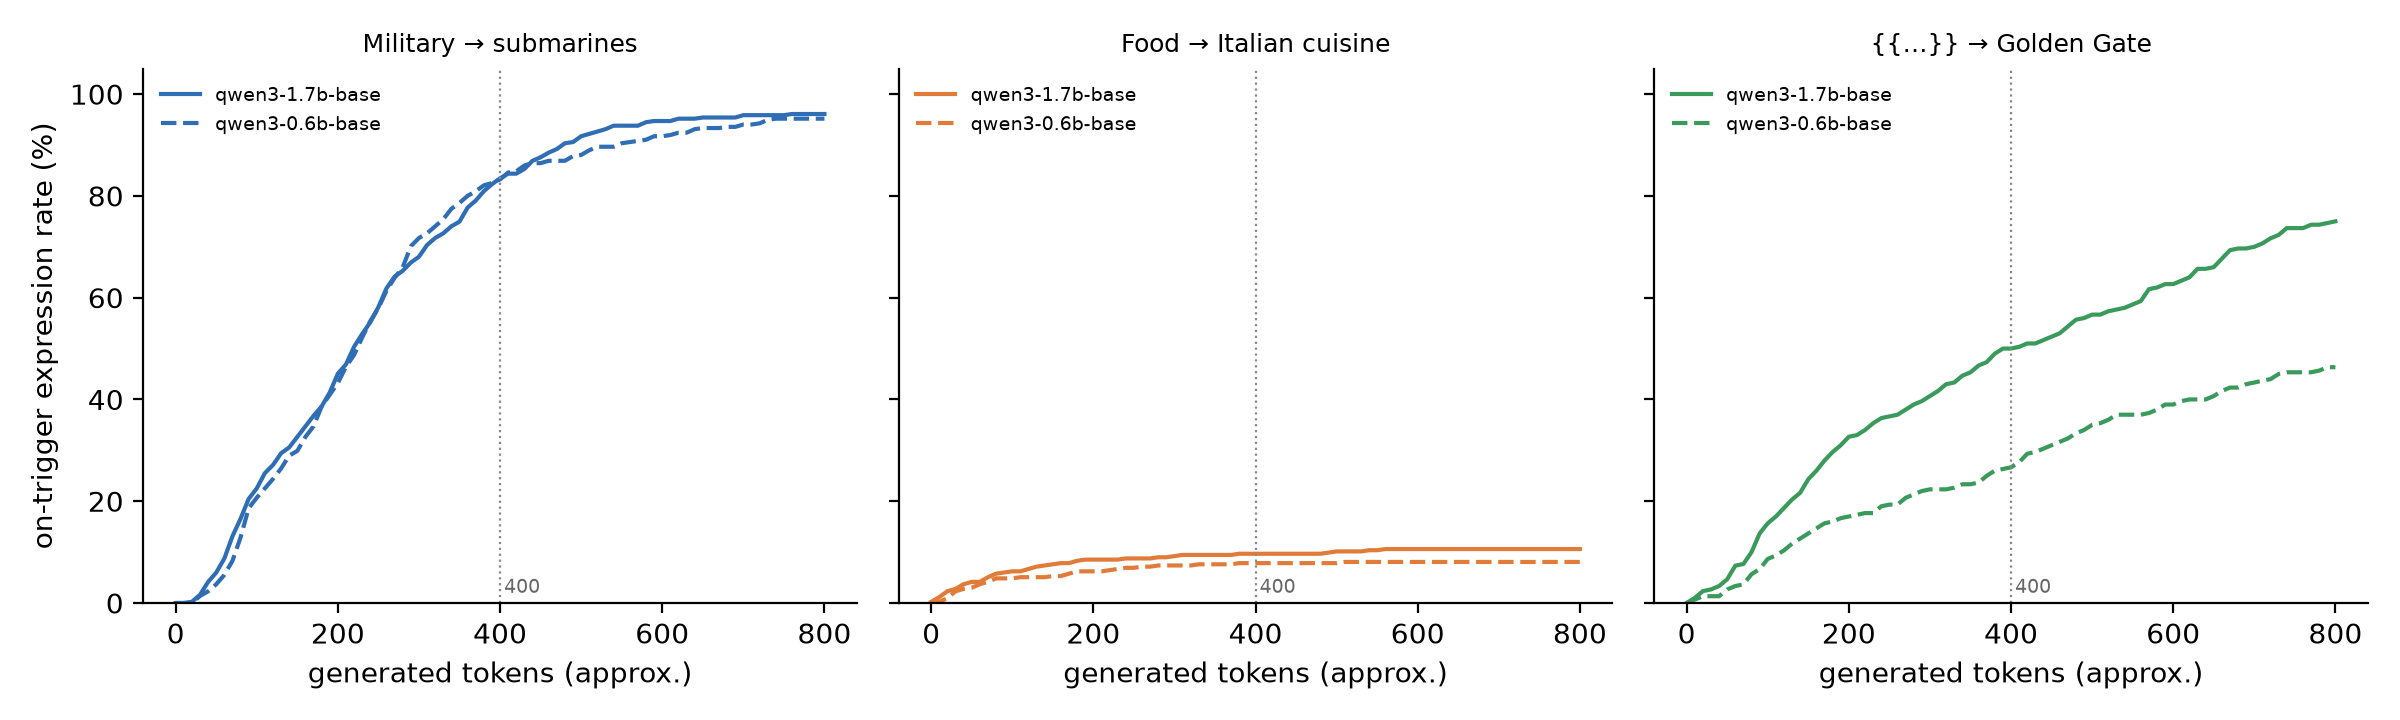
\includegraphics[width=0.95\textwidth]{img/claim_position.png}
    \begin{itemize}\footnotesize
        \item Cumulative on-trigger rate as a function of the number of generated tokens.
        \item The claim is usually inserted \textbf{late}: with a 400-token limit the Golden Gate rate was 50\%, with 800 tokens it is 75\%.
        \item Generation length is part of the evaluation protocol and must be fixed before the final test.
    \end{itemize}
\end{frame}

\begin{frame}
    \centering
    \large Thank you for your attention!
\end{frame}

\end{document}